\documentclass[10pt,a4paper,twocolumn]{article}

\usepackage[a4paper,top=18mm,bottom=21mm,left=17mm,right=17mm,columnsep=6mm]{geometry}
\usepackage[T1]{fontenc}
\usepackage[utf8]{inputenc}
\usepackage{lmodern}
\usepackage{microtype}
\usepackage{booktabs}
\usepackage{array}
\usepackage{graphicx}
\usepackage{xcolor}
\usepackage{caption}
\usepackage{tikz}
\usetikzlibrary{arrows.meta,positioning,fit,backgrounds}
\usepackage{natbib}
\usepackage{hyperref}
\usepackage{fancyhdr}

\definecolor{ink}{HTML}{172033}
\definecolor{muted}{HTML}{5B6472}
\definecolor{blue}{HTML}{2563A6}
\definecolor{orange}{HTML}{D97706}
\definecolor{pale}{HTML}{F2F5F8}
\hypersetup{colorlinks=true,linkcolor=blue,citecolor=blue,urlcolor=blue,pdfauthor={Umut Yunus Yesildal},pdftitle={Transfer or Relearning? Work-in-Progress Paper}}
\captionsetup{font=small,labelfont=bf}
\setlength{\parindent}{1em}
\setlength{\parskip}{0pt}
\renewcommand{\arraystretch}{1.12}
\emergencystretch=1.5em

\pagestyle{fancy}
\fancyhf{}
\fancyhead[L]{\footnotesize\color{muted}WORK IN PROGRESS --- INTERNAL DRAFT}
\fancyhead[R]{\footnotesize\color{muted}9 August 2026}
\fancyfoot[C]{\footnotesize\thepage}
\renewcommand{\headrulewidth}{0.3pt}

\newcommand{\mzero}{M0}
\newcommand{\mone}{M1}
\newcommand{\mta}{M2-A}
\newcommand{\mtb}{M2-B}
\newcommand{\trtoen}{TR$\rightarrow$EN}
\newcommand{\enttoen}{EN$\rightarrow$EN}
\newcommand{\trtotr}{TR$\rightarrow$TR}
\newcolumntype{L}[1]{>{\raggedright\arraybackslash}p{#1}}
\newcommand{\wipbox}[1]{\noindent\colorbox{pale}{\parbox{0.96\columnwidth}{\small\textbf{WIP boundary.} #1}}}

\title{\vspace{-1.2em}\textbf{Transfer or Relearning?}\\[-0.1em]
\large A Controlled Synthetic-Fact Study of Cross-Lingual Access after Turkish Continued Pretraining}
\author{Umut Yunus Yesildal\\\small Master's Thesis Work-in-Progress}
\date{9 August 2026}

\begin{document}
\twocolumn[{
\begin{@twocolumnfalse}
\maketitle
\vspace{-1.1em}
\begin{abstract}
When a language model becomes better able to answer factual questions in a target language, the gain may reflect cross-lingual access to previously learned knowledge, renewed learning from target-language data, or both. We study this distinction using fictitious subject--relation--object facts whose exposure history is controlled. The completed work establishes a replicated English acquisition state in Qwen2.5-1.5B over 500 subjects and 2,500 facts, then compares two equal-budget Turkish continued-pretraining arms initialized independently from the same English-acquired model: a fact-free arm and an arm containing four controlled exposure cycles for the 1,250 Branch-B facts. Across two seeds, Turkish prompting with English answers fell by 18.75 and 18.83 percentage points after fact-free adaptation. Controlled factual re-exposure recovered 1.86 and 1.89 points relative to the fact-free sibling. However, the precommitted Branch-B-specific interaction was $+0.25$ points (95\% CI $[-0.51,1.01]$) for seed 42 and $+1.35$ points (95\% CI $[0.51,2.18]$) for seed 43. Because both independent seeds were required to pass, the frozen primary criterion was not met. We present this as a complete, negative/inconclusive Qwen Wikipedia-only 1M-token pilot, not as a final answer to the thesis question. The paper also documents the acquisition diagnostics that made the causal test possible and motivates a prospective literature-first design with source-model provenance, broader Turkish data, and explicit language-adaptation manipulation checks.
\end{abstract}
\vspace{0.7em}
\wipbox{This draft reports only completed and independently checked evidence. The next literature-first experiment is prospective and remains blocked by unresolved measurement-design and corpus-selection gates.}
\vspace{1.1em}
\end{@twocolumnfalse}
}]

\section{Introduction}

Multilingual language models do not provide uniform factual access across languages. Factual recall varies with the language of inquiry, semantically equivalent prompts can produce inconsistent rankings, and multilingual surface competence does not guarantee deeper cross-lingual knowledge access \citep{schott2023polyglot,qi2023crosslingual,chua2025barriers,aggarwal2025inquiry}. Mechanistic and longitudinal work further suggests that factual representations can be partly shared while access and output mapping remain language-sensitive \citep{zhao2024roots,wang2025lost,liu2025acquisition}.

This creates an identification problem for target-language adaptation. Suppose a model is first taught a fact in English and later answers it from a Turkish question. If the Turkish adaptation corpus contained the same fact, success need not be transfer: it may be reaffirmation or relearning. Conversely, a null result is uninterpretable when the adaptation did not demonstrably improve Turkish modeling. Naturally occurring facts worsen this problem because their multilingual pretraining history is unknown.

We address the exposure problem with fictitious facts and matched sibling adaptation arms. The project makes four current contributions:

\begin{enumerate}
  \item a controlled synthetic-fact and candidate-ranking framework that separates canonical storage, prompt-robust retrieval, relation binding, and cross-lingual access;
  \item a documented acquisition ladder showing why exact memorization and low training loss are insufficient preconditions for a transfer study;
  \item a complete two-seed, 2,500-fact Qwen pilot comparing fact-free Turkish adaptation with controlled Turkish factual re-exposure; and
  \item a transparent negative/inconclusive primary result that motivates stronger source-model, corpus, and manipulation-check controls rather than post-hoc threshold or checkpoint search.
\end{enumerate}

The central finding is asymmetric. English factual retention remained high, yet fact-free Turkish continued pretraining sharply reduced Turkish-prompt access to the English-acquired answers. Factual re-exposure recovered a small fraction of the loss, but its precommitted Branch-specific effect did not replicate across both seeds.

\section{Related Work}

\paragraph{Multilingual factual access.}
Prior work establishes cross-language inconsistency in factual knowledge, language-of-inquiry effects, and barriers that remain even when models show translation competence \citep{qi2023crosslingual,schott2023polyglot,chua2025barriers,aggarwal2025inquiry}. Tracing studies distinguish facts learned independently, shared across languages, or transferred from a source language \citep{zhao2024roots}; other work follows the emergence of multilingual factual knowledge during pretraining \citep{liu2025acquisition}. \citet{wang2025lost} argue that inconsistency can arise at multiple stages, including mapping internally available knowledge to a target-language output space. These studies motivate direction-specific measurements, but they do not isolate target-language adaptation with known fact exposure.

\paragraph{Controlled knowledge acquisition.}
Fictitious datasets such as TOFU illustrate how synthetic entities can control whether information was present in training \citep{maini2024tofu}. Controlled biographies show that extraction quality depends strongly on training-data diversity and cannot be inferred from storage alone \citep{allenzhu2023storage}. Our setting uses synthetic facts for a different purpose: source attribution across English acquisition and Turkish adaptation.

\paragraph{Target-language adaptation and forgetting.}
Turkish adaptation work demonstrates that target-language data, model choice, tokenizer efficiency, and dose all matter \citep{acikgoz2024bosphorus}. Continual multilingual learning also exposes catastrophic-forgetting trade-offs \citep{winata2023forgetting,yamaguchi2026shielded}. Domain-adaptation work shows that within-language acquisition and cross-language transfer can follow different dynamics \citep{zhao2026dynamics}. We therefore track source-language factual retention and generic language modeling separately from Turkish-prompt factual access.

\paragraph{Turkish corpus and tokenizer evidence.}
Turkish model development provides several corpus precedents rather than a single obvious adaptation source. Prior work has trained compact encoders on mixed Turkish data and studied OSCAR-specific tokenization \citep{kesgin2023turkishbert,toraman2023tokenization}, trained monolingual decoder models \citep{kesgin2024cosmosgpt}, used the vngrs web corpus for Turkish sequence-to-sequence pretraining \citep{turker2024vbart}, and combined mC4, OSCAR, and Wikipedia for large Turkish encoders \citep{schmitt2026sindbert}. Multilingual releases such as HPLT and FineWeb2 broaden the auditable candidate pool \citep{arefyev2024hplt,penedo2025fineweb2}. These studies establish feasibility and emphasize corpus composition and tokenizer fit, but their architectures and objectives do not identify factual transfer in our causal setting.

\section{Question and Causal Design}

The thesis asks:

\begin{quote}
When factual knowledge becomes retrievable through Turkish after Turkish adaptation, does this reflect cross-lingual access to English-acquired knowledge, or additional reaffirmation/relearning caused by Turkish factual exposure?
\end{quote}

Figure~\ref{fig:design} shows the design. \mone{} acquires every synthetic fact in English. Two Turkish arms then start independently from the same frozen \mone{} endpoint. The historical artifact names are \texttt{M2-clean} and \texttt{M3-fact}; conceptually, we refer to them as \mta{} and \mtb{} because they are parallel siblings, not sequential stages.

\begin{figure*}[t]
\centering
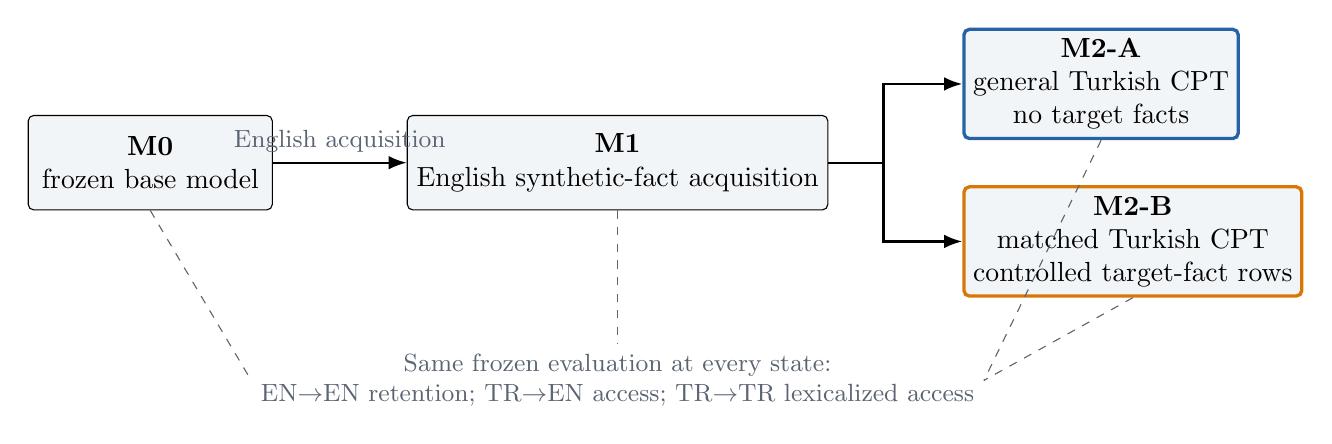
\begin{tikzpicture}[
  node distance=9mm and 17mm,
  box/.style={draw,rounded corners=2pt,minimum width=31mm,minimum height=12mm,align=center,fill=pale},
  armA/.style={box,draw=blue,very thick},
  armB/.style={box,draw=orange,very thick},
  arr/.style={-{Latex[length=2.3mm]},thick},
  note/.style={align=center,font=\small,color=muted}
]
\node[box] (m0) {\textbf{\mzero{}}\\frozen base model};
\node[box,right=of m0] (m1) {\textbf{\mone{}}\\English synthetic-fact acquisition};
\node[armA,right=of m1,yshift=10mm] (m2a) {\textbf{\mta{}}\\general Turkish CPT\\no target facts};
\node[armB,right=of m1,yshift=-10mm] (m2b) {\textbf{\mtb{}}\\matched Turkish CPT\\controlled target-fact rows};
\draw[arr] (m0) -- node[above,note]{English acquisition} (m1);
\draw[arr] (m1.east) -- ++(7mm,0) |- (m2a.west);
\draw[arr] (m1.east) -- ++(7mm,0) |- (m2b.west);
\node[note,below=17mm of m1] (eval) {Same frozen evaluation at every state:\\ \enttoen{} retention; \trtoen{} access; \trtotr{} lexicalized access};
\draw[dashed,color=muted] (m0.south) -- (eval.west);
\draw[dashed,color=muted] (m1.south) -- (eval.north);
\draw[dashed,color=muted] (m2a.south) -- (eval.east);
\draw[dashed,color=muted] (m2b.south) -- (eval.east);
\end{tikzpicture}
\caption{Causal design. Both Turkish arms are initialized independently from the same frozen \mone{} model and receive equal total token/update budgets. In the completed pilot, only Branch-B facts were repeated in \mtb{}, enabling a Branch difference-in-differences.}
\label{fig:design}
\end{figure*}

For the completed pilot, Branch A and Branch B receive identical English acquisition. \mta{} contains no target synthetic binding. \mtb{} repeats only the 1,250 Branch-B facts; Branch A receives zero Turkish factual exposures. The frozen primary estimand is therefore
\[
  \bigl(\mathrm{M2\mbox{-}B}-\mathrm{M2\mbox{-}A}\bigr)_{B,\,\mathrm{TR\to EN}}
  - \bigl(\mathrm{M2\mbox{-}B}-\mathrm{M2\mbox{-}A}\bigr)_{A,\,\mathrm{TR\to EN}}.
\]
This controls for generic differences between the two trained siblings. A positive average \mtb{}--\mta{} difference alone is descriptive, not the confirmatory test.

\section{Synthetic Facts and Evaluation}

\subsection{Relation V2 inventory}

The canonical inventory contains 5,000 synthetic subjects, five relations per subject, and 25,000 facts. The present pilot uses a balanced intermediate subset of 500 subjects: 250 Branch A and 250 Branch B, for 2,500 facts. The five relations are \texttt{profession}, \texttt{born\_in}, \texttt{lives\_in}, \texttt{field\_of\_study}, and \texttt{works\_in\_industry}. \texttt{born\_in} and \texttt{lives\_in} deliberately share a city inventory, making same-subject relation swaps visible.

Earlier proper-name-heavy relations, \texttt{studied\_at} and \texttt{works\_at}, caused candidate-prior and tokenization collapse. Relation V2 replaced them with balanced short-answer inventories and independently assigned candidates. This redesign was methodological, not outcome-driven at the final pilot stage.

\subsection{Candidate ranking and robustness}

For each prompt, the evaluator scores every candidate object in the frozen relation inventory by mean answer-token log probability. Top-1 accuracy asks whether the gold object outranks all relation-matched alternatives. This avoids free-generation spelling and alias normalization as primary confounds, but limits the claim to factual access among a frozen candidate set.

Four prompt forms (A--D) are crossed with direct-question and Question/Answer scaffolds. A fact is ``eight-cell robust'' only when it is top-1 in all eight form/scaffold cells. The evaluator also records same-subject relation-swapped forced choice, generic WikiText-2 perplexity \citep{merity2017wikitext}, empty/short output behavior, and synthetic-subject intrusion.

The bilingual endpoint evaluation uses three directions:
\begin{itemize}
  \item \enttoen{}: English storage and post-adaptation retention;
  \item \trtoen{}: primary cross-lingual access with the English object surface; and
  \item \trtotr{}: access plus Turkish answer lexicalization.
\end{itemize}
Each state has $3\times4\times2=24$ slices and 2,500 probes per slice, or 60,000 probe rows. The four Turkish endpoints produced 96/96 complete slices; the two frozen \mone{} anchors yield six matched 60,000-row state tables.

\subsection{Uncertainty and gates}

Outcomes are averaged within subject and resampled with 2,000 subject-bootstrap draws using frozen seed 20260717. The primary gate required, in \emph{both} independent seed chains, an observed Branch interaction above zero and a 95\% bootstrap lower bound above zero. The \enttoen{} guardrail required every Turkish endpoint to remain within five percentage points of its seed-matched \mone{} state.

\section{Establishing a Usable \mone{}}

The project did not assume that low training loss or canonical exact accuracy implied transferable knowledge. Table~\ref{tab:development} summarizes the main diagnostic progression.

\begin{table*}[t]
\centering
\small
\caption{Selected methodological milestones. Values are retained evidence, not a unified leaderboard; populations and evaluators differ by row.}
\label{tab:development}
\begin{tabular}{@{}L{30mm}L{25mm}L{39mm}L{65mm}@{}}
\toprule
Stage & Scale/model & Key observation & Consequence \\
\midrule
M0 baseline & 100 subjects & Direct and QA top-1 both 0.6\% & Synthetic bindings were not detectably accessible before acquisition. \\
Early broad recipes & GPT-2 / SmolLM & Low direct/QA retrieval despite low loss, richer biographies, repetition, QA mixing, and two-stage training & Broad recipe search was replaced by a diagnostic acquisition ladder. \\
Direct-aware micro ladder & 1, 10, then 50 facts & Held-out direct/QA access became near-perfect at small scale & Prompt-family coverage and answer-focused supervision were necessary. \\
SmolLM2-360M scale test & 500 vs. 2,500 facts & Exact storage stayed 99.92\% at 2,500 facts, but direct/QA overlap fell to 38.3\% & Canonical storage and robust retrieval were separated as distinct gates. \\
SmolLM2-1.7B controls & 500 facts & Simple direct/QA retrieval approached ceiling, but held-out subject forms and generic retention exposed form dependence and drift & Forms C/D, eight-cell robustness, PPL, EOS, and binding diagnostics became mandatory. \\
Qwen2.5-1.5B selected \mone{} & 2,500 facts; seeds 42/43 & Eight-cell robust 96.08/96.20\%; exact 99.96/99.68\%; PPL/base 1.082/1.032 & Seed-42 step 75 and seed-43 step 50 were frozen under the earliest-all-gates rule. \\
\bottomrule
\end{tabular}
\end{table*}

The selected Qwen \mone{} condition used 17,500 factual rows, answer-only factual loss, clean-English replay with coefficient 0.5, 36 epochs, physical batch 50, gradient accumulation 50, and 252 optimizer updates. Eleven checkpoints were evaluated. Rather than choosing the numerically strongest point, the frozen rule selected the earliest checkpoint passing every exact, cell, robust, binding, PPL, and integrity gate: step 75 for seed 42 and step 50 for seed 43. These checkpoints achieved 99.51\% and 99.56\% relation forced choice and 29/30 generic-completion top-1, with zero synthetic-subject intrusion.

\section{Completed Qwen Wikipedia-Only Pilot}

\subsection{Training contract}

Each selected \mone{} seed spawned two independent Turkish continual-pretraining runs. Both arms used 512-token pretokenized blocks, 2,048 blocks, 1,048,576 total tokens, 128 optimizer updates, learning rate $10^{-5}$, the same batch decomposition, data seed, scheduler, and fixed endpoint \texttt{checkpoint-128}. The general Turkish material came from the frozen \texttt{trwiki-20260601} corpus.

\mta{} contained zero target factual exposure. \mtb{} replaced matched material with four complete cycles over the 1,250 Branch-B facts, for 5,000 scheduled factual exposures. Branch A remained unexposed in Turkish. Equal total tokens and updates prevent the fact arm from receiving a larger optimization budget.

\subsection{Execution integrity}

All four training runs completed. Endpoint evaluation eventually produced all 96 registered Turkish-arm slices. Failed GPU allocations and a pending-task commit-guard mismatch occurred before evaluator execution; only missing slices were retried. Strict assembly checked completion markers, hashes, row counts, unique probe IDs, registry membership, and static metadata before analysis. An independent read-only review recomputed the primary bootstrap and retention comparisons from the per-probe state tables and returned \emph{PASS WITH CONCERNS}; its concerns were a stale pre-execution status label and a timed-out home-directory capacity scan, not scientific inconsistencies.

\section{Results}

\subsection{State-level factual access}

Figure~\ref{fig:states} and Table~\ref{tab:states} give the frozen headline results. Before Turkish adaptation, \mone{} already showed about 52\% \trtoen{} and 29--30\% \trtotr{} access. Fact-free Turkish adaptation did not open further access: \trtoen{} fell to 33.29\% and 33.70\%, declines of 18.75 and 18.83 points. \trtotr{} fell by 6.59 and 6.87 points.

\begin{figure*}[t]
\centering
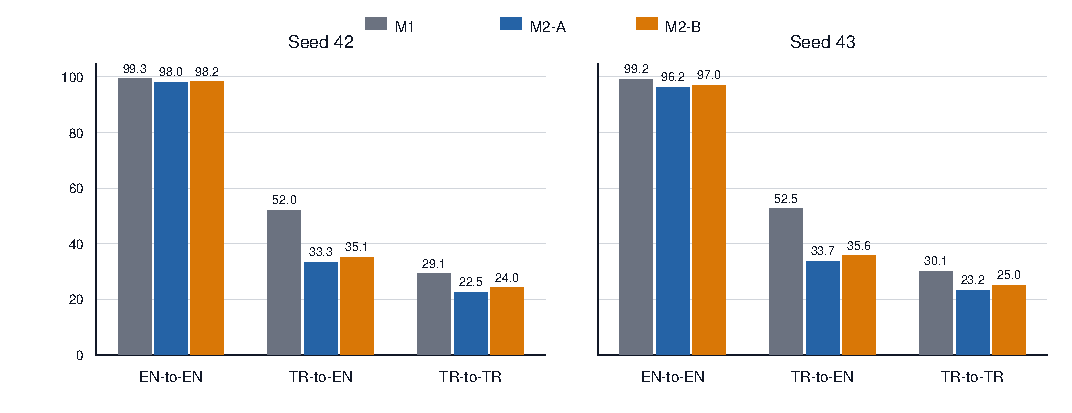
\includegraphics[width=0.90\textwidth]{figures/headline_state_accuracy.pdf}
\caption{Frozen top-1 accuracy for the two seed chains. \mta{} corresponds to the historical \texttt{M2-clean} arm and \mtb{} to \texttt{M3-fact}. Turkish adaptation preserved most \enttoen{} access but sharply reduced both Turkish-prompt directions.}
\label{fig:states}
\end{figure*}

\begin{table*}[t]
\centering
\small
\caption{Frozen endpoint top-1 accuracy with 95\% subject-bootstrap confidence intervals (2,000 draws; 500 subjects per state).}
\label{tab:states}
\begin{tabular}{llccc}
\toprule
Seed & State & \enttoen{} & \trtoen{} & \trtotr{} \\
\midrule
42 & \mone{} & 99.29 [99.14, 99.43] & 52.03 [50.89, 53.19] & 29.05 [27.90, 30.20] \\
42 & \mta{} & 98.05 [97.72, 98.36] & 33.29 [32.07, 34.48] & 22.46 [21.36, 23.50] \\
42 & \mtb{} & 98.22 [97.94, 98.48] & 35.14 [33.96, 36.33] & 24.04 [22.94, 25.08] \\
\addlinespace
43 & \mone{} & 99.24 [99.04, 99.42] & 52.52 [51.18, 53.82] & 30.12 [28.97, 31.21] \\
43 & \mta{} & 96.24 [95.54, 96.87] & 33.70 [32.43, 34.90] & 23.25 [22.18, 24.30] \\
43 & \mtb{} & 96.95 [96.37, 97.45] & 35.59 [34.33, 36.81] & 24.97 [23.87, 26.10] \\
\bottomrule
\end{tabular}
\end{table*}

\subsection{Primary interaction}

Relative to its matched \mta{} sibling, \mtb{} improved \trtoen{} by 1.86 points (95\% CI [1.48, 2.22]) for seed 42 and 1.89 points ([1.48, 2.33]) for seed 43. \trtotr{} improved by 1.58 and 1.72 points. These consistent arm-level differences are descriptive because Branch A also changed modestly between independently trained siblings.

The confirmatory Branch interaction was much smaller for seed 42: $+0.25$ points, CI $[-0.51,1.01]$. Seed 43 showed $+1.35$ points, CI $[0.51,2.18]$. Figure~\ref{fig:effects} makes the distinction explicit. The seed-42 interval crosses zero, so the required two-seed primary criterion was not met.

\begin{figure}[t]
\centering
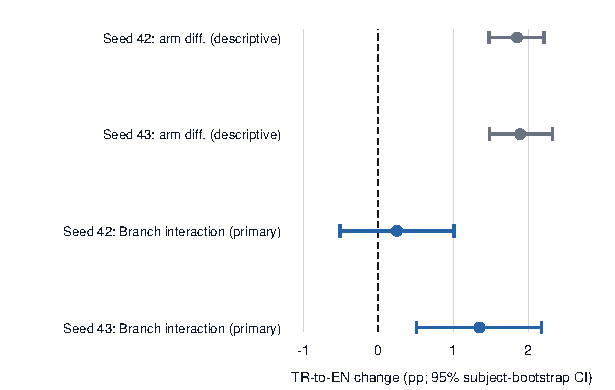
\includegraphics[width=\columnwidth]{figures/primary_effects.pdf}
\caption{Descriptive sibling-arm changes and the precommitted Branch interaction. Only the Branch interaction is the completed pilot's primary causal test.}
\label{fig:effects}
\end{figure}

\subsection{Retention and exploratory structure}

The \enttoen{} retention guardrail passed. The worst endpoint was seed-43 \mta{} at $-3.00$ points relative to \mone{}, within the frozen $-5$-point limit. Thus the dominant loss was not broad erasure of English factual knowledge.

Post-hoc analysis found the largest \trtoen{} losses in \texttt{profession}, \texttt{works\_in\_industry}, and \texttt{lives\_in}. Both direct and QA scaffolds and all four forms showed the same qualitative decline and modest recovery; form C was most vulnerable. \mtb{} restored only roughly one tenth of the preceding \trtoen{} loss. These subgroup patterns are exploratory and do not alter the primary gate.

\section{Discussion}

\paragraph{Turkish CPT did not imply improved factual access.}
The clean arm changed the model while preserving most English access, yet Turkish-prompt factual ranking deteriorated sharply. This separates target-language exposure from preservation of a previously open bilingual access path. The effect is stable across seeds and directions involving Turkish prompts.

\paragraph{Factual re-exposure provided limited recovery.}
The fact arm outperformed the clean sibling in both seeds, so controlled re-exposure was not behaviorally inert. However, only seed 43 showed a confidence-bounded Branch-B-specific effect. The appropriate conclusion is not ``relearning succeeded,'' but that re-exposure was associated with a small descriptive recovery whose precommitted causal replication criterion failed.

\paragraph{The source model complicates a transfer claim.}
Qwen2.5 is a multilingual base model \citep{qwen25modelcard}. Its \mone{} state already achieved about 52\% \trtoen{} before Turkish CPT. The pilot therefore probes preservation and modification of an existing bilingual access path as much as the emergence of a new one. It cannot support the stronger claim that an English-only model learned Turkish access from scratch.

\paragraph{Acquisition validity matters upstream.}
The development history shows that exact completion accuracy can coexist with severe form dependence. A transfer experiment built on canonical memorization alone would confound language access with prompt-specific English acquisition. The replicated Qwen \mone{} state passed a much stronger eight-cell, relation-binding, PPL, and integrity contract, making the downstream negative result interpretable within the pilot's limits.

\section{Limitations}

\begin{enumerate}
  \item \textbf{Source-language provenance.} Qwen's Turkish pretraining share is not known, and the model is explicitly multilingual.
  \item \textbf{Adaptation dose and corpus.} Each arm received only 1,048,576 Turkish Wikipedia tokens. This is narrow and far below many published target-language adaptation regimes \citep{acikgoz2024bosphorus}. The literature-first primary corpus has not yet been selected or materialized.
  \item \textbf{Incomplete manipulation checks.} Endpoint Turkish PPL and an independent base-compatible Turkish capability measure were not part of the frozen primary package. A factual null cannot cleanly distinguish failed language adaptation from failed transfer.
  \item \textbf{Candidate ranking.} The evaluator establishes access among frozen candidates, not unrestricted generation. \trtotr{} additionally depends on alias localization.
  \item \textbf{Scale and replication.} The pilot uses 500 subjects, 2,500 facts, and two seeds. The historical 25,000-fact inventory was not run in this causal family.
  \item \textbf{Treatment decomposition.} The completed family lacks a lexical/entity-only arm. Its Branch interaction controls generic sibling differences but cannot separately estimate entity alignment.
  \item \textbf{Exploratory analyses.} Relation, form, scaffold, and recovery-fraction analyses were performed after the frozen result and remain hypothesis-generating.
\end{enumerate}

\section{Prospective Literature-First Study}

The next experiment is deliberately separated from the completed pilot. No result is reported in this section.

\paragraph{Source-model audit.}
An English-centric base model with documented training provenance and measurable Turkish headroom should be compared with Qwen as a multilingual positive control. Candidate claims must distinguish ``documented English-only,'' ``Turkish not listed,'' and ``Turkish exposure unknown'' rather than asserting forensic absence of Turkish web contamination.

\paragraph{Corpus and dose.}
The frozen Wikipedia corpus remains a high-provenance cross-domain control, not the prospective primary corpus. The paper-backed candidate pool includes vngrs, Turkish OSCAR and mC4 derivatives, HPLT, and FineWeb2 \citep{toraman2023tokenization,turker2024vbart,schmitt2026sindbert,arefyev2024hplt,penedo2025fineweb2}. A publication precedent does not make an exact snapshot selected or training-ready: the final source must pass revision, license, route, language-ID, usable-text, duplication, privacy/noise, target-fact contamination, and evaluation-overlap audits. In the current project state, vngrs is only a conditional materialization candidate, Turkish Wikipedia is control-only, CulturaX is access-blocked, and the additional candidates remain unaudited. Dose must be selected using fact-free adaptation and frozen language measures before observing factual-treatment outcomes.

\paragraph{Manipulation checks.}
Within-model Turkish PPL should be paired with a tokenizer-normalized measure such as bits per character or byte for cross-model comparisons. A base-compatible grammar or minimal-pair diagnostic should complement broader Turkish knowledge/reasoning benchmarks such as audited subsets of CETVEL or TurkBench \citep{er2026cetvel,toraman2026turkbench}. English PPL and \enttoen{} retention remain guardrails.

\paragraph{Matched sibling contrast.}
The prospective \mta{} and \mtb{} arms must start from the same frozen \mone{}, use identical general-corpus order, tokenizer, total tokens, optimizer updates, replay ratio if any, and endpoint rule. Target-fact rows in \mtb{} replace matched neutral Turkish tokens rather than increasing the training budget. The principal factual outcome remains \trtoen{}; \trtotr{} is secondary and EN$\rightarrow$TR is exploratory.

At the time of this draft, corpus selection/materialization and exact measurement design remain unresolved. The project is not ready to measure or train this new family, and no prospective claim is included in the results.

\section{Reproducibility and Research Practice}

Every selected model, dataset, slice registry, aggregate table, and gate is bound by manifests and SHA-256 hashes. Failed jobs and corrections are retained chronologically rather than rewritten. The completed endpoint package contains 96/96 Turkish-arm slices and six matched 60,000-row state tables; independent recalculation reproduced the primary estimates. The four endpoint models were frozen as model-only copies with 24/24 retained files passing checksum verification.

The synthetic subjects are fictitious, reducing privacy and natural-fact provenance concerns. Web-corpus work introduces licensing, personal-data, harmful-content, and benchmark-contamination risks; these are explicit acceptance gates for the prospective study. High-volume artifacts are kept on scratch storage, while compact manifests, checksums, and result summaries preserve the scientific record.

\section{Conclusion}

This work establishes a controlled route from English factual acquisition to a two-arm Turkish adaptation test. The Qwen \mone{} state robustly acquired 2,500 English facts in two seeds. In the completed Wikipedia-only 1M-token pilot, fact-free Turkish CPT substantially reduced Turkish-prompt access while largely preserving English factual retrieval. Controlled Turkish factual re-exposure produced a small, consistent descriptive recovery, but the Branch-specific primary effect passed in only one seed. The frozen conclusion is therefore negative/inconclusive: the primary success criterion was not met.

The result is scientifically useful because it rules out a simple narrative in which any Turkish continued pretraining automatically opens cross-lingual factual access. A stronger next test requires a better documented source model, broader audited Turkish data, and direct evidence that the language-adaptation manipulation worked before transfer and relearning are compared.

\section*{Draft Status}

This is a work-in-progress synthesis through 9 August 2026. It is not a submission-ready manuscript and does not supersede frozen experiment manifests or chronological result reports. The completed pilot result is fixed; the prospective experiment remains unexecuted.

\bibliographystyle{plainnat}
\bibliography{references}

\end{document}
